\documentclass[12pt]{article}
\usepackage[utf8]{inputenc}
\usepackage[spanish,es-tabla]{babel}
\usepackage[square,sort,comma,numbers]{natbib}
\usepackage{amssymb,amsmath,amsthm,amsfonts}
\usepackage{calc}
\usepackage{gensymb}
\usepackage{natbib}
\usepackage{url}
\usepackage{amsmath}
\usepackage{graphicx}
\usepackage{parskip}
\usepackage{fancyhdr}
\usepackage{vmargin}
\usepackage[table,xcdraw]{xcolor}
\usepackage[top=2cm,bottom=2cm]{geometry}
\usepackage{graphicx}
\usepackage{pdflscape}
\usepackage{caption}
%\usepackage{subfigure}
\usepackage{xurl}
\usepackage{booktabs}
\usepackage{subfig}
\usepackage{float}
%Agregados
\usepackage[shortlabels]{enumitem}

\def\BibTeX{{\rm B\kern-.05em{\sc i\kern-.025em b}\kern-.08em
    T\kern-.1667em\lower.7ex\hbox{E}\kern-.125emX}}
\setmarginsrb{3 cm}{2.5 cm}{3 cm}{2.5 cm}{1 cm}{1.5 cm}{1 cm}{1.5 cm}

\title{Ejercicio N$^{\circ}$1}					 % Titulo
\author{Elias Obreque \\ Gustavo Ceballo \\ Maibeth Sánchez}					 % Autor
\date{\today}						% Fecha


\makeatletter
\let\thetitle\@title
\let\theauthor\@author
\let\thedate\@date
\makeatother

\pagestyle{fancy}
\fancyhf{}
\lhead{\thetitle}
\cfoot{\thepage}

\begin{document}

%%%%%%%%%%%%%%%%%%%%%%%%%%%%%%%%%%%%%%%%%%%%%%%%%%%%%%%%%%%%%%%%%%%%%%%%%%%%%%%%%%%%%%%%%

\begin{titlepage}
	\centering
    \vspace*{0.0 cm}
    
\includegraphics[scale = 0.13]{Logo_Uchile_modern.png}\\[1.0 cm]	% Logo Universidad
    \textsc{\LARGE Universidad de Chile}\\[2.0 cm]	% Nombre Universidad
	\textsc{\Large EL7012}\\[0.5 cm]				 % Codigo Curso
	\textsc{\large Control Inteligente de Sistemas, Otoño}\\[0.2 cm]		 % Nombre Curso
	\rule{\linewidth}{0.2 mm} \\[0.2 cm]
	{ \huge \bfseries \thetitle}\\
	\rule{\linewidth}{0.2 mm} \\[0.5 cm]
	
	\begin{minipage}{0.4\textwidth}
		\begin{center} \large
			\emph{Autor:}\\
			\theauthor\linebreak
			\end{center}
	\end{minipage}\\[1.5 cm]
	
	{\large \thedate}\\[1.5 cm]

	\vfill
	
\end{titlepage}

%%%%%%%%%%%%%%%%%%%%%%%%%%%%%%%%%%%%%%%%%%%%%%%%%%%%%%%%%%%%%%%%%%%%%%%%%%%%%%%%%%%%%%%%%

\tableofcontents

\thispagestyle{empty}
\pagebreak
\newpage
\setcounter{page}{1}

%%%%%%%%%%%%%%%%%%%%%%%%%%%%%%%%%%%%%%%%%%%%%%%%%%%%%%%%%%%%%%%%%%%%%%%%%%%%%%%%%%%%%%%%%

\section{Introducción}

La  mayoría  de  los  sistemas  tienen  un  comportamiento  no  lineal,  excepto  en  un determinado rango de operación donde pueden ser considerados lineales. En ocasiones un modelo lineal es insuficiente para explicar un fenómeno por lo que se debe recurrir a Modelos No Lineales.

Los modelos basados en redes neuronales y sistemas difusos han sido empleados para la identificación, dado que han mostrado una grancapacidad para aproximar funciones no lineales desconocidas, además de que ofrecen una estructura general tan compleja o sencilla como el problema lo demande. Por un lado, las redes neuronales son estructuras matemáticas inspiradas en las estructuras biológicas compuestas por neuronas, en donde a través de elementos relativamente simples (llamados neuronas)que efectúan operaciones y procesos muy sencillos logran, mediante interconexiones, realizarprocesos complejos y procesamiento de información en paralelo. En general se consideran redes neuronales conformadas por “capas” de neuronas, donde una capa procesa la información recibida en paralelo y la envía a la siguiente capa de neuronas. Por otro lado, los sistemas difusos son también estructuras matemáticas, aunque estos se encuentran inspirados en los procesos de pensamiento y toma de decisiones llevados a cabo por los humanos, así como en la teoría de conjuntos difusos propuesta por Lofti Zadeh.

En este ejercicio se dará solución al Problema 1.


\subsection{Problema 1}

Considere la siguiente serie no lineal dinámica:

\begin{align}
y(k)= (0.8 - 0.5 exp\{-y^2(k- 1)\})y(k - 1)\nonumber \\
-(0.3 + 0.9 exp\{-y^2(k - 1)\})y(k - 2)\nonumber \\
+u(k - 1) + 0.2u(k - 2) + 0.1u(k - 1)u(k - 2) + e(k)
\label{e_serie}
\end{align}

donde el ruido del sistema

\begin{equation}
e(k)=  0.5 exp\{-y^2(k- 1)\}\beta(k)
\label{e_error}
\end{equation}

depende del estado previo de la salida del modelo, y $\beta(k)$ es un ruido blanco.

Como usted sabe existen varias técnicas que se pueden emplear para la modelación a partir de estos datos, por lo que debe seleccionar el tipo de modelo más adecuado para este tipo de sistema. Para este trabajo se le pide detallar la metodología utilizada para:

\begin{enumerate}[a)]
\item Generar 600 datos a partir de esta serie. Considere 55\% para entrenamiento, 25\% test y 20\% validación.
\item Obtener un modelo de predicción lineal, difuso tipo-1 (T\&S) y neuronal para la salida. Evaluar las predicciones a 1, 8 y 16 pasos. Comparar el desempeño de todos los modelos a partir de las métricas más apropiadas tales como RMSE, MAPE, MAE, entre otras. Comente.
\item Construir el intervalo de predicción de los modelos obtenidos en b) utilizando el método de la covarianza.
\item Evaluar los intervalos de predicción obtenidos en b) realizando predicciones a 1, 8, y 16 pasos. Comparar el desempeño de los modelos a partir de las métricas más apropiadas tales como ancho del intervalo, probabilidad de cobertura, entre otras.
\item Construir el intervalo de predicción del modelo difuso encontrado en a) con el método de optimización min-max. Compare este intervalo de predicción con el intervalo obtenido utilizando el método de la covarianza. Comente.
\item Construir el intervalo de predicción neural utilizando el método de Joint Supervision. Compare con los métodos anteriores.
\item Seleccione el modelo más apropiado y justifique.
\end{enumerate}

\newpage
\section{Generación de Datos}

En esta estapa es necesario generar datos que representen la dinámica del sistema en la mayor cantidad de rangos de operación posibles, ya que el modelo obtenido tiene un ancho de banda acotado, y por lo tanto las dinámicas definidas por fuera de dicha banda podrían no ser representadas adecuadamente. Para lo cual se debe diseñar una entrada $u(k)$ que excite a la planta en el rango de frecuencias en que se encuentran los fenómenos de interés.

En este trabajo se propone el uso de señales binarias pseudo aleatorias (Pseudo Random Binary Signal, PRBS),  ya  que  es  una  de  las  señales  más  utilizadas  en  identificación  de sistemas. Esta es una señal periódica, determinística y que  posee  principalmente  propiedades  similares  al  ruido  blanco  (contenido  muy  rico  en frecuencias)

Para general la señal se suponen los siguientes parámetros de interés $f_{min}=0.2 Hz$, $f_{max}=1 Hz$ y tiempo de muestreo $T_S=0.01$. Con los parámetros anteriores, y utilizando la expresión

\begin{equation}
n=\frac{log(f_c/f_{min}+1)}{log(2)})
\label{e_}
\end{equation}

con $f_c=2.5*f_{max}=2.5 Hz$, se genera una PRBS de orden $n= 4$, por lo que el largo máximo corresponde a $N = 2^n - 1 = 15$. A su vez, la cantidad de muestras por bit son $N_{s} = 40$. Luego, el tiempo de un bit, $\triangle t=N_s*T_s=0.4s$, por lo que la PRBS dura en total 6s y debe ser replicada 400 veces con diferentes condiciones iniciales para obtener los 6000 datos de interés. Finalmente se genera la APRBS variando la amplitud aleatoriamente de la PRBS generada, Fig.\ref{f_APRBS} y se aplica a la serie no lineal como se muestra en la Fig.\ref{f_SerieNoLineal}.

\begin{figure}
\centering
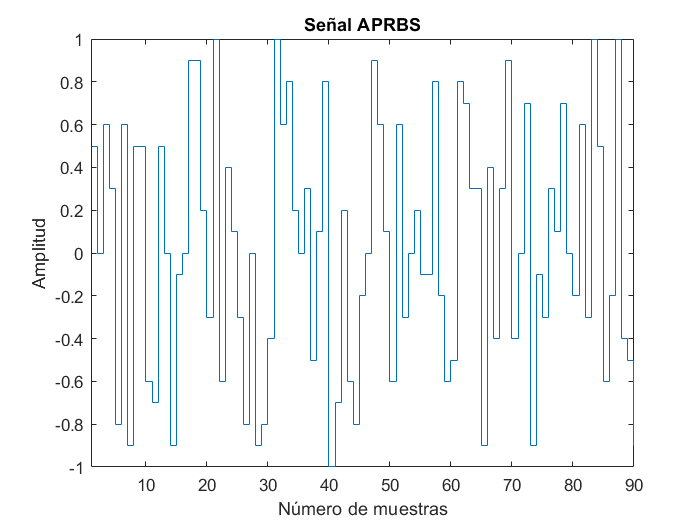
\includegraphics[width=10cm,height=7cm]{imag/APRBS}
\caption{Señal APRBS con Amplitud entre -1 y +1.}
\label{f_APRBS}
\end{figure}

\begin{figure}
\centering
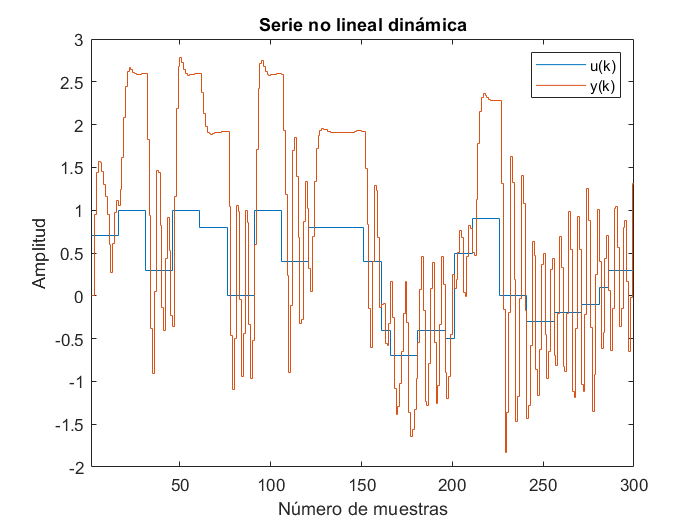
\includegraphics[width=10cm,height=7cm]{imag/SerieNoLineal}
\caption{Respuesta de la serie no lineal.}
\label{f_SerieNoLineal}
\end{figure}


Una vez obtenidos los datos experimentales de entrada-salida, éstos son clasificados en tres conjuntos con distinta información: datos de entrenamiento, datos
de validación y datos de prueba; esto con el fin de evaluar adecuadamente los modelos
generados. El conjunto de entrenamiento se utiliza para determinar los parámetros del
modelo. El conjunto de prueba permite comparar distintas estructuras de los modelos
generados. Finalmente, el conjunto de validación permite verificar el sobreajuste del
modelo óptimo obtenido, evaluándolo en un nuevo conjunto de datos (distintos a los
datos del conjunto de entrenamiento y validación), analizando su capacidad de
generalización. En este caso se utiliza una división de 55\% de los datos para entrenamiento, 25\% para prueba y 20\% validación.

\section{Modelos de predicción}
\subsection{Modelo lineal}

En este caso, supondremos que se ajustará un modelo lineal suponiendo que el sistema real es lineal con ruido blanco gaussiano aditivo, es decir,


\begin{equation}
y(k)=a_1 y(k-1)+a_2 y(k-2)+b_1 u(k-1)+b_2 u(k-2)+e(k)
\label{e_ModeloLineal}
\end{equation}

Luego, se propone un modelo lineal para llevar a cabo la predicción a 1 paso, de modo tal que:

Predicción a 1 paso:

\begin{equation}
\hat{y}(k)=\hat{a}_1 y(k-1)+\hat{a}_2 y(k-2)+\hat{b}_1 u(k-1)+\hat{b}_2 u(k-2)
\label{e_Pre1paso}
\end{equation}

Este modelo no considera un valor constante o bias dao el supuesto que el sistema es lineal con ruido blanco aditivo. En caso que se sospechara que existe un bias o tendencia (trend) en el sistema, se puede agregar otro vector de unos a la matriz de regresores (o matriz de información).

Para llevar a cabo la estimación de los parámetros del modelo se utilizó la técnica de mínimos cuadrados, es decir:

\begin{equation}
\hat{\theta}=(Xent^T*Xent)^{-1}*Xent^T*\hat{y}(k)
\label{e_AjustMinCuadrados}
\end{equation}


En que $\hat{\theta}=[\hat{a}_1 \quad \hat{a}_2 \quad \hat{b}_1 \quad \hat{2}_2]^T$ es el vector de parámetros y $Xent$ es la matriz de regresores con los valores de las $n$ muestras ordenados por filas.

Los valores que se obtuvieron de los parámetros fueron los siguientes:


\begin{equation}
\hat{\theta}=\left(
                \begin{array}{c}
                  \hat{a}_1  \\
                  \hat{a}_2  \\
                  \hat{b}_1  \\
                  \hat{b}_2  \\
                \end{array}
              \right)
=\left(
   \begin{array}{c}
     0.8601 \\
     -0.6930 \\
     0.9724 \\
     0.3486 \\
   \end{array}
 \right)
\label{e_ValoresCoeficientes}
\end{equation}

A continuación, en la Tabla \ref{t_NoLinealp1}, se presentan las métricas de bondad del ajuste o errores en los diversos conjuntos de datos, a saber, conjunto de datos de entrenamiento, prueba o test y validación.


% Table generated by Excel2LaTeX from sheet 'Sheet1'
\begin{table}[htbp]
  \centering
  \caption{Errores o Métricas de bondad de ajuste a 1 paso}
    \begin{tabular}{|p{4.055em}|r|r|r|}
    \toprule
    Métricas & \multicolumn{1}{p{6.11em}|}{Conjunto Entrenamiento} & \multicolumn{1}{p{5.61em}|}{Conjunto de Prueba} & \multicolumn{1}{p{5.055em}|}{Conjunto de Validación} \\
    \midrule
    RMSE  & 0.0115 & 0.019 & 0.0241 \\
    \midrule
    MAPE  & 123.1323 & 101.9383 & 169.4761 \\
    \midrule
    MAE   & 0.3313 & 0.3402 & 0.3524 \\
    \bottomrule
    \end{tabular}%
  \label{t_NoLinealp1}%
\end{table}%

\newpage

\subsection{Modelo difuso Takagi-Sugeno Tipo-1}

\begin{itemize}
	\item \textbf{Selección de variables}:
Para seleccionar las variables que actúan como entrada al sistema difuso, se realiza un análisis de sensibilidad. Suponiendo una estructura del modelo inicial difuso con 8 variables de entrada $y(k-1)$,..., $y(k-4)$, $u(k-1)$,...,$u(k-4)$. En la Fig. \ref{f_P1Sensibilidad} se muestran los índices de las sensibilidades del modelo inicial para las 8
variables de entrada, comprobándose que las variables las variables $y(k-4)$, $u(k-3)$ y $u(k-4)$ presentan menores índices de las sensibilidades, por lo cual no son incluidos en el modelo difuso. A pesar de que los regresores $y(k-3)$ y $u(k-2)$ presentan una sensibilidad similar se decidio escoger $u(k-1)$ ya que el mismo es un parámetro de la serie no lineal dinámica.

\begin{figure}
\centering
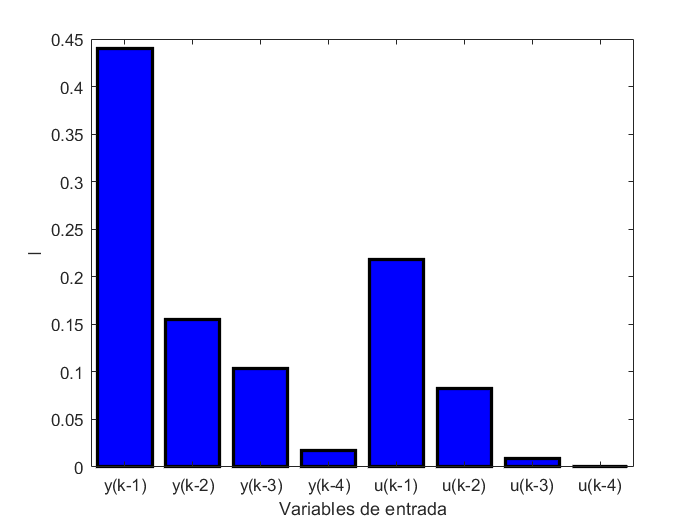
\includegraphics[width=10cm,height=7cm]{imag/P1Sensibilidad}
\caption{Índice de Sensibilidades.}
\label{f_P1Sensibilidad}
\end{figure}

La Tabla \ref{t_Error} indica el valor de la Raíz del Error Cuadrático Medio (RMSE) para los modelos con 8 y 4 regresores, y se puede notar que son muy semejantes, y por consiguiente se eselecciona el modelo más sencillo.

\begin{equation}
RMSE=\sqrt{\frac{1}{N}\sum_{k=1}^{N}(y(k)-y_{fuzzy}(k))^2}
\label{e_RMSE}
\end{equation}


donde $N$ es la cantidad total de datos, $y(k)$ es la salida de la planta real en el instante $k$ , e $y_{fuzzy}(k)$ es la predicción realizada por el modelo difuso en el instante $k$.

% Table generated by Excel2LaTeX from sheet 'Sheet1'
\begin{table}[htbp]
  \centering
  \caption{Índices de Error para el Análisis de Sensibilidades.}
    \begin{tabular}{|r|l|r|}
    \toprule
    \multicolumn{1}{|p{4.055em}|}{Modelo } & \multicolumn{1}{p{5.555em}|}{Variables de entrada } & \multicolumn{1}{p{4.055em}|}{RMSE} \\
    \midrule
    1     & $y(k-1)$,$y(k-2)$,$y(k-3)$,$y(k-4)$, & 0.2177 \\
    & $u(k-1)$,$u(k-2)$,$u(k-3)$,$u(k-4)$ & \\
    \midrule
    2     & $y(k-1)$,$y(k-2)$,$u(k-1)$,$u(k-2)$    & 0.2109 \\
    \bottomrule
    \end{tabular}%
  \label{t_Error}%
\end{table}%

\item \textbf{Optimización de la estructura}:
La optimización de la estructura del modelo difuso consiste principalmente en determinar el número óptimo de reglas del modelo difuso. En este caso se definió un número máximo de 20 clusters y se entrenó el modelo para cada una de las posibles valores de clusters, utilizando como algoritmo de clustering el Fuzzy C-Means.

La Fig. \ref{f_P1reglas11} muestra el RMSE para los conjuntos de entrenamiento y prueba.  Si no importa la complejidad, el mejor modelo es aquel que
tiene menor RMSE. Sin embargo, es posible que un modelo con peor índice de
desempeño, pero menos complejo que el modelo óptimo, pueda obtener resultados
aceptables bajo un estándar de rendimiento definido preliminarmente. Por lo antes expuesto para este problema se escoge como número de clusters 5, por lo que el modelo difuso contará con 5 reglas, Fig \ref{f_Cluster}.

\begin{figure}
\centering
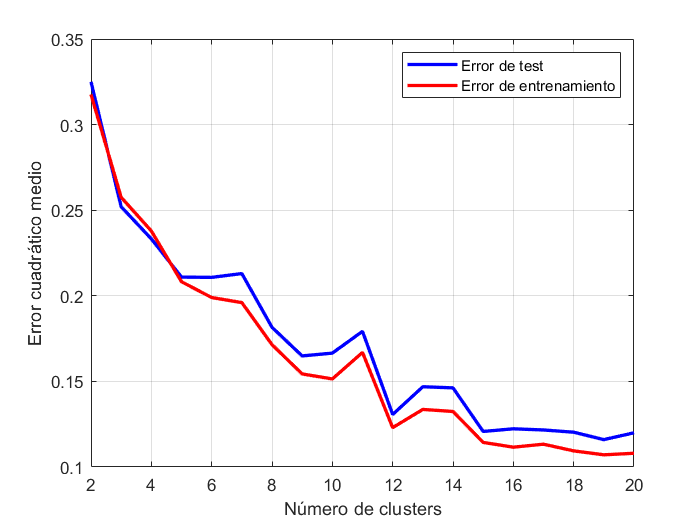
\includegraphics[width=10cm,height=7cm]{imag/P1reglas12}
\caption{Índice de Sensibilidades.}
\label{f_P1reglas11}
\end{figure}

Además del RMSE, se pueden definir el Error Porcentual Absoluto Medio (MAPE, Mean Absolute Percentage Error) y Error Absoluto Medio (MAE, Mean Absolute Error) para comprobar el modelo difuso obtenido.

\begin{equation}
MAPE=\frac{1}{N}\sum_{k=1}^{N}\frac{y(k)-y_{fuzzy}(k)}{y(k)}
\label{e_MAPE}
\end{equation}

\begin{equation}
MAE=\frac{1}{N}\sum_{k=1}^{N}|y(k)-y_{fuzzy}(k)|
\label{e_MAE}
\end{equation}


% Table generated by Excel2LaTeX from sheet 'Sheet1'
\begin{table}[htbp]
  \centering
  \caption{Índices de Error para el Modelo Difuso}
    \begin{tabular}{|l|r|r|r|}
    \toprule
    Índices & \multicolumn{3}{c|}{Conjunto} \\
\cmidrule{2-4}          & \multicolumn{1}{l|}{Entrenamiento} & \multicolumn{1}{p{6em}|}{Prueba} & \multicolumn{1}{p{6.39em}|}{Validación} \\
    \midrule
    RMSE  & 0.2082 & 0.2109 & 0.1938 \\
    \midrule
    MAPE  & 70.92 & 65.65 & 67.71 \\
    \midrule
    MAE   & 0.1454 & 0.1505 & 0.1344 \\
    \bottomrule
    \end{tabular}%
  \label{t_MD}%
\end{table}%

En la Tabla \ref{t_MD} se puede ver como el RMSE se mantiene de similar para los conjuntos de prueba y validadación lo que indica la capacidad de generalización del modelo. Por su parte el índice MAPE, mide el tamaño del error (absoluto) en términos porcentuales, indicando que el error porcentual promedio del modelo se encuentra alrededor del 70\%, si bien este es un valor grande, es válido destacar que see sta trabajando con una señal cuya salida se encuentra entre [-2,3]. El MAE tampoco presenta variaciones entre los diferentes conjuntos de datos. Considerando un compromiso entre complejidad y desempeño se determina que el modelo propuesto con 4 regresores y 5 reglas es suficiente.

\begin{figure}
		\centering
		\captionsetup{justification=centering}
		\subfloat[Salida]{
		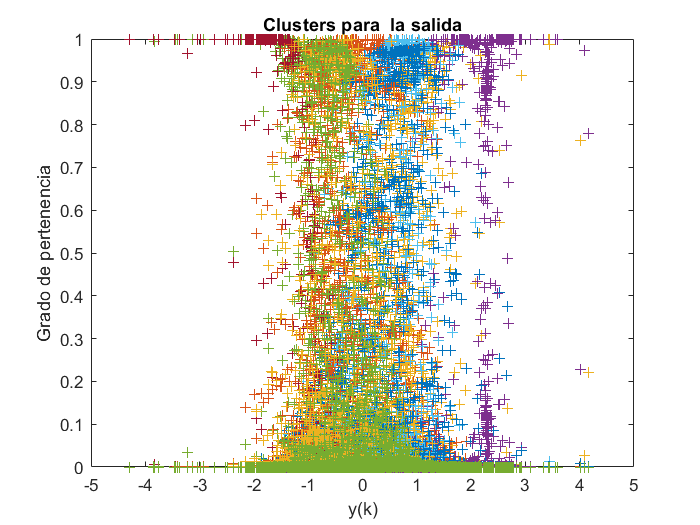
\includegraphics[width=0.5\textwidth]{imag/ClusterSalida}}\\
		\subfloat[$y(k-1)$]{
		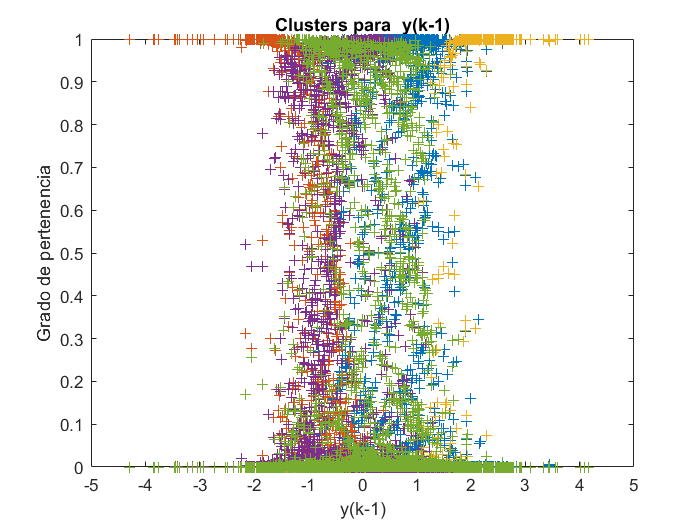
\includegraphics[width=0.5\textwidth]{imag/Clustery1}}
		\subfloat[$y(k-2)$]{
		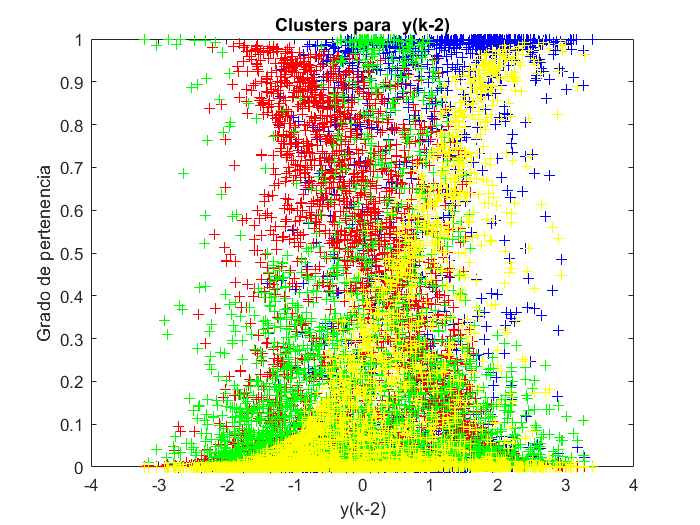
\includegraphics[width=0.5\textwidth]{imag/Clustery2}}\\
        \subfloat[$u(k-1)$]{
		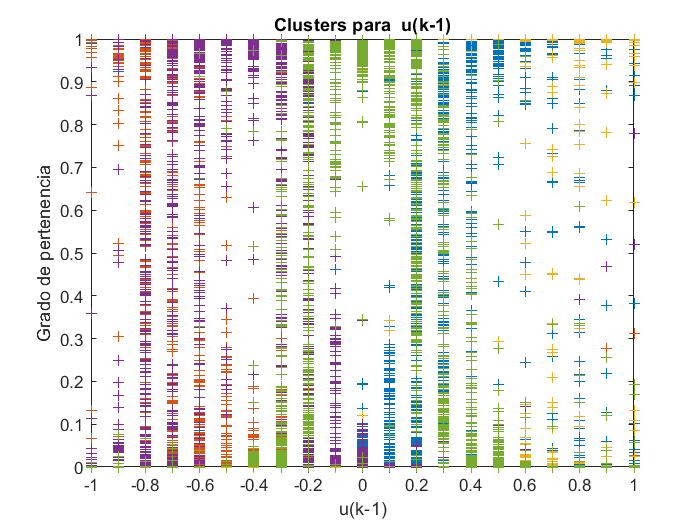
\includegraphics[width=0.5\textwidth]{imag/Clusteru1}}
		\subfloat[$u(k-2)$]{
		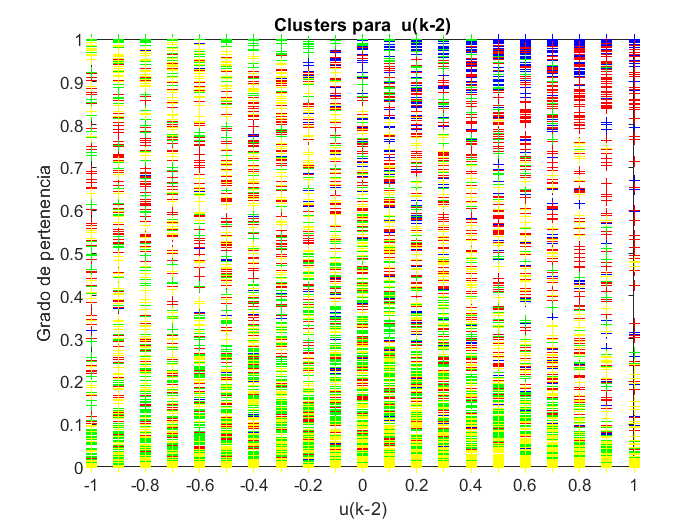
\includegraphics[width=0.5\textwidth]{imag/Clusteru2}}
		\caption{Clusters del Modelo Difuso Tipo 1.}
		\label{f_Cluster1}
\end{figure}

\item \textbf{Optimización de los parámetros}: Se utiliza el algortimo de clustering difuso Fuzzy C-Means obteniéndose siguientes parámetros de los consecuentes, de dimensión $[N_Rx\theta]$

\begin{equation}
\left(
  \begin{array}{ccccc}
 -0.1625 &	0.99755	&-0.7451	&0.8430	 &0.2983\\
0.4561&	1.1500	& -0.3126	&0.5930	& 0.1362\\
-0.2139&	0.8892&	-0.2883&	1.0148&	0.2207\\
-0.10934&	0.8182&	-0.9810&	0.6261&	0.1752\\
0.0032&	0.5939&	-0.9615&	1.0893&	0.3707
  \end{array}
\right)
\label{e_ParaModDif}
\end{equation}

\item \textbf{Predicciones a 1, 8, y 16
pasos}:

Las Fig. \ref{f_SalidaModelo} muestra la salida del modelo difuso y  la estimación para 1, 8 y 16 pasos respectivamente.

\begin{figure}
		\centering
		\captionsetup{justification=centering}
		\subfloat[Salida del Modelo]{
		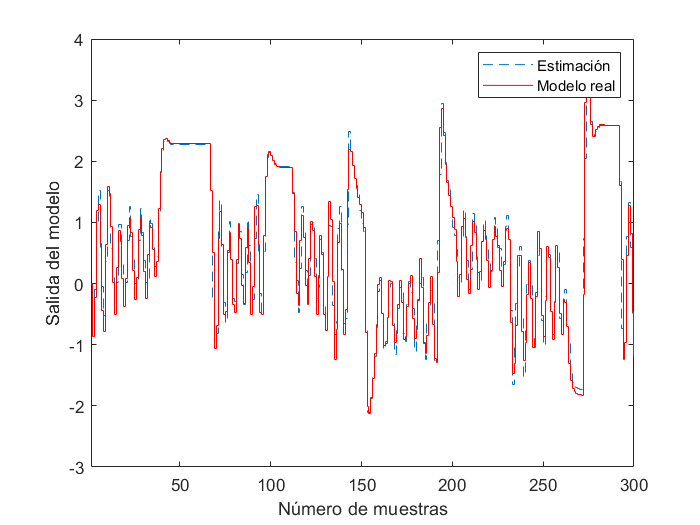
\includegraphics[width=0.5\textwidth]{imag/P1SalidaZoom}}
		\subfloat[Salida del modelo a 1 paso]{
		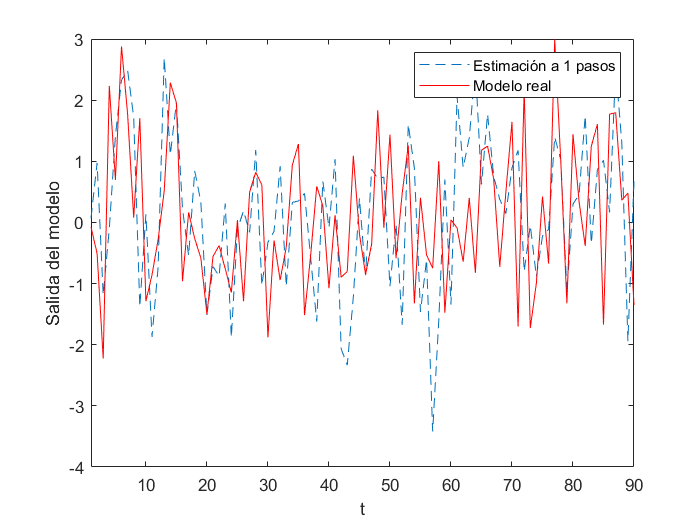
\includegraphics[width=0.5\textwidth]{imag/P1Salida_p1Zoom}}\\
        \subfloat[Salida del modelo a 8 pasos]{
		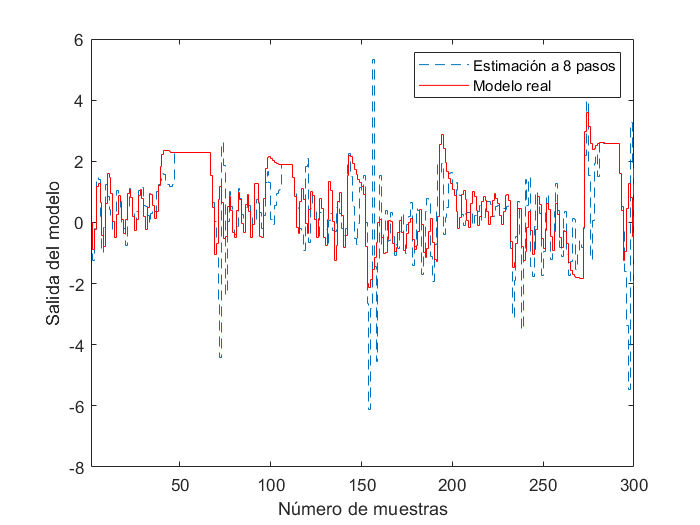
\includegraphics[width=0.5\textwidth]{imag/P1Salida_p8Zoom}}
		\subfloat[Salida del modelo a 16 pasos]{
		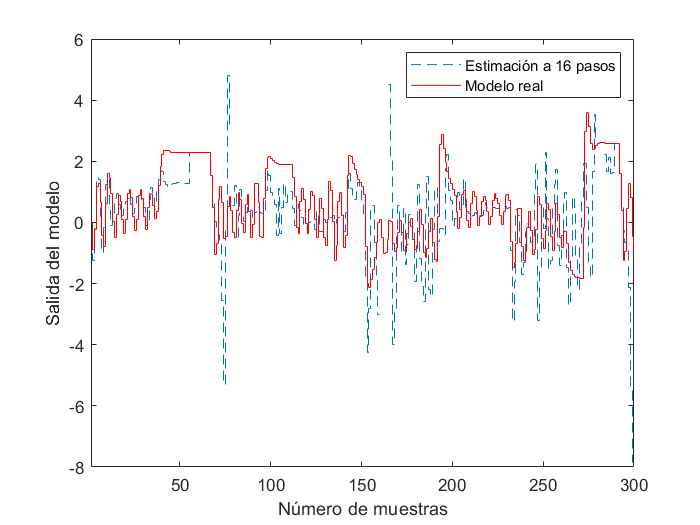
\includegraphics[width=0.5\textwidth]{imag/P1Salida_p16Zoom}}
		\caption{Respuesta del Modelo Difuso Tipo 1.}
		\label{f_SalidaModelo}
\end{figure}


En la Tabla \ref{t_MDjp} se establece una comparación entre los modelos obtenidos, como se puede comprobar a amedida que aumenta el paso de la estimación el desempeño de del modelo difuso se deteriora.

% Table generated by Excel2LaTeX from sheet 'Sheet1'
\begin{table}[htbp]
  \centering
  \caption{Desempeño del Modelo difuso a j-pasos}
    \begin{tabular}{|l|r|r|r|r|}
    \toprule
    Índices & \multicolumn{4}{c|}{Modelos} \\
\cmidrule{2-5}          & \multicolumn{1}{l|}{Estimado} & \multicolumn{1}{p{6em}|}{Predicción a 1 pasos} & \multicolumn{1}{p{6.39em}|}{Predicción a 8 pasos} & \multicolumn{1}{p{5.445em}|}{Predicción a 16 pasos} \\
    \midrule
    RMSE  & 0.1938 & 0.2432 & 0.7077 & 0.8847 \\
    \midrule
    MAPE  & 67.71 & 108.72 & 159.78 & 169.81 \\
    \midrule
    MAE   & 0.1344 & 0.1816 & 0.5076 & 0.6814 \\
    \bottomrule
    \end{tabular}%
  \label{t_MDjp}%
\end{table}%

\item \textbf{Covarianza}:

\begin{figure}
		\centering
		\captionsetup{justification=centering}
		\subfloat[Salida del modelo. Método de la Covarianza]{
		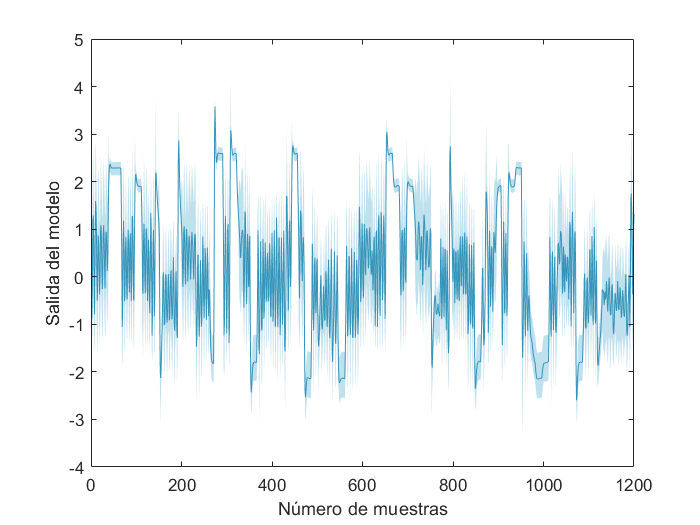
\includegraphics[width=0.5\textwidth]{imag/P1Covarianza}}
		\subfloat[Salida del modelo a 1 paso]{
		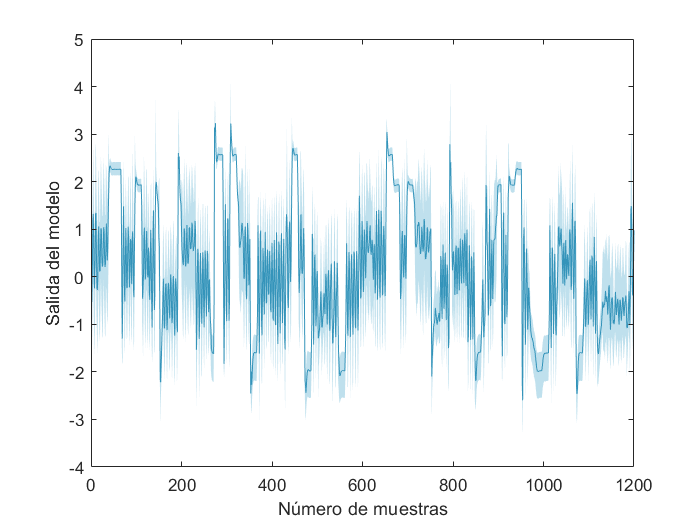
\includegraphics[width=0.5\textwidth]{imag/P1Covarianza_p1}}\\
        \subfloat[Salida del modelo a 8 pasos]{
		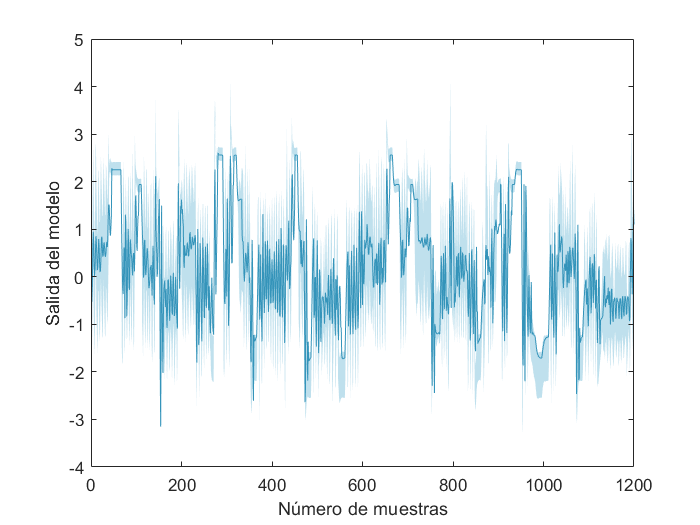
\includegraphics[width=0.5\textwidth]{imag/P1Covarianza_p8}}
		\subfloat[Salida del modelo a 16 pasos]{
		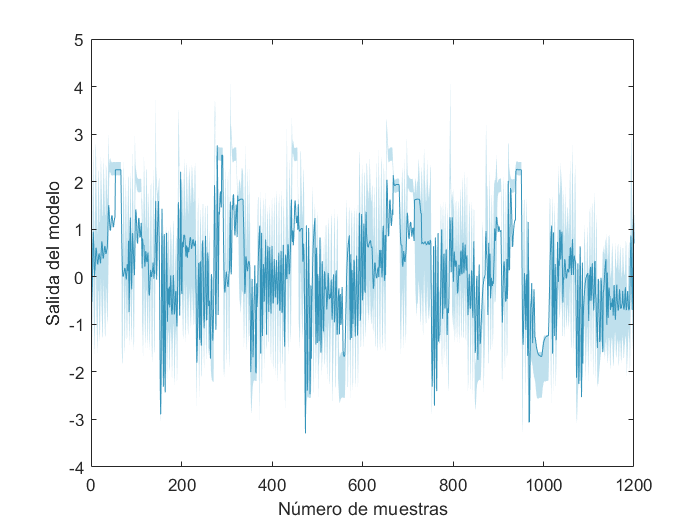
\includegraphics[width=0.5\textwidth]{imag/P1Covarianza_p16}}
		\caption{Intervalo difuso. Método de la Covarianza.}
		\label{f_P1Covarianza}
\end{figure}



% Table generated by Excel2LaTeX from sheet 'Sheet1'
\begin{table}[htbp]
  \centering
  \caption{Intervalos de predicción. Método de la Covarianza}
    \begin{tabular}{|l|r|r|r|r|}
    \toprule
    Índices & \multicolumn{4}{c|}{Modelos} \\
\cmidrule{2-5}          & \multicolumn{1}{l|}{Estimado} & \multicolumn{1}{p{6em}|}{Predicción a 1 pasos} & \multicolumn{1}{p{6.39em}|}{Predicción a 8 pasos} & \multicolumn{1}{p{5.445em}|}{Predicción a 16 pasos} \\
    \midrule
    PICP  & 100   & 99.33 & 84.67 & 72 \\
    \midrule
    PINAW & 27.59 & 29.2  & 29.55 & 28.1 \\
    \bottomrule
    \end{tabular}%
  \label{tab:addlabel}%
\end{table}%



\item \textbf{MinMax}:

\begin{figure}
		\centering
		\captionsetup{justification=centering}
		\subfloat[Salida del modelo. Método de la Covarianza]{
		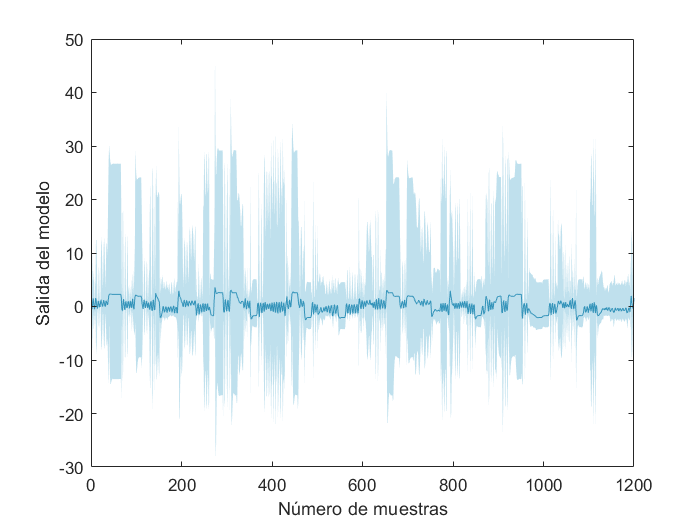
\includegraphics[width=0.5\textwidth]{imag/P1MinMax}}
		\subfloat[Salida del modelo a 1 paso]{
		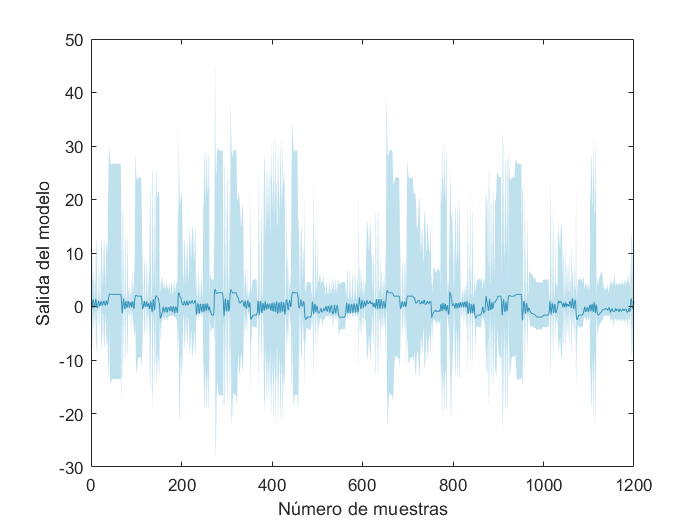
\includegraphics[width=0.5\textwidth]{imag/P1MinMax_p1}}\\
        \subfloat[Salida del modelo a 8 pasos]{
		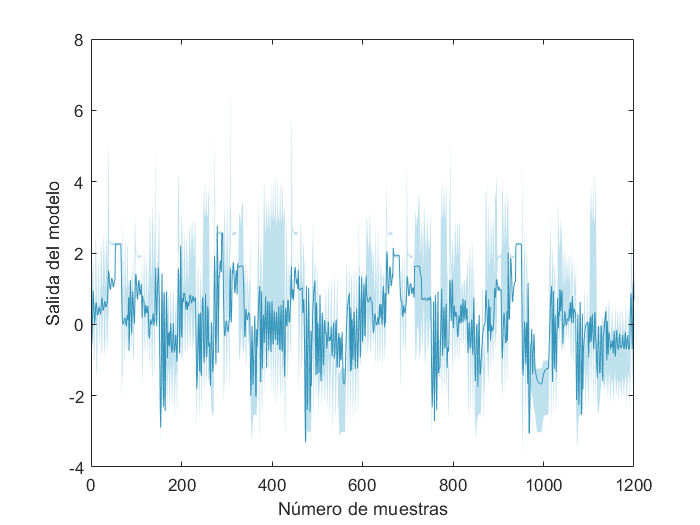
\includegraphics[width=0.5\textwidth]{imag/P1MinMax_p8}}
		\subfloat[Salida del modelo a 16 pasos]{
		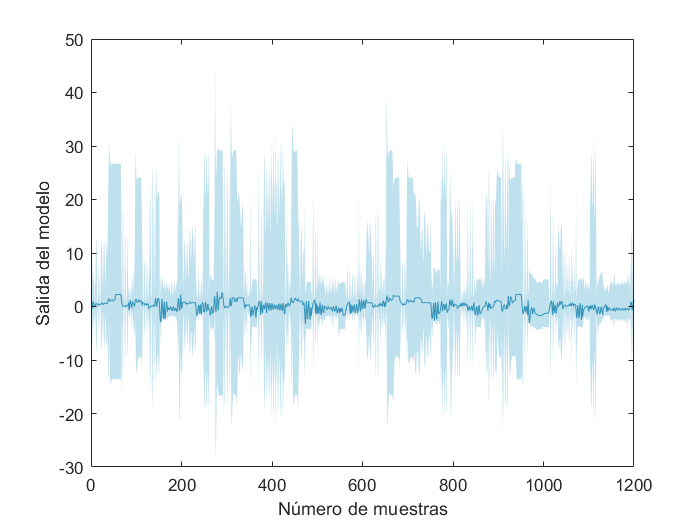
\includegraphics[width=0.5\textwidth]{imag/P1MinMax_p16}}
		\caption{Intervalo difuso. Método MinMax}
		\label{f_P1MinMax}
\end{figure}






% Table generated by Excel2LaTeX from sheet 'Sheet1'
\begin{table}[htbp]
  \centering
  \caption{Intervalos de predicción. Método MinMax}
    \begin{tabular}{|l|r|r|r|r|}
    \toprule
    Índices & \multicolumn{4}{c|}{Modelos} \\
\cmidrule{2-5}          & \multicolumn{1}{l|}{Estimado} & \multicolumn{1}{p{4.055em}|}{Predicción a 1 pasos} & \multicolumn{1}{p{4.055em}|}{Predicción a 8 pasos} & \multicolumn{1}{p{4.055em}|}{Predicción a 16 pasos} \\
    \midrule
    PICP  & 98.5  & 98.08 & 96.42 & 95.67 \\
    \midrule
    PINAW & 296.69 & 313.96 & 317.784 & 302.19 \\
    \bottomrule
    \end{tabular}%
  \label{tab:addlabel}%
\end{table}%


\end{itemize}


\newpage
\subsection{Modelo de red neuronal}

Para encontrar un buen modelo de red neuronal se propone seguir los pasos de identificación.

\begin{itemize}
	\item \textbf{Obtención de datos:} Para ello se utiliza el set de datos creado en el punto a) del problema.
	\item \textbf{Selección de datos:} Análogo a los modelos anteriores, se utilizan los datos repartido con un 55\% en el conjunto de entrenamiento, 25\% en el conjunto de prueba y 20\% en el conjunto de validación.
	\item \textbf{Definición de la estructura de la red:} Se propone una red con una capa oculta, función de activación \textit{tanh} en la salida de la capa oculta y algoritmo de aprendizaje Levenberg-Marquardt. Las variables de entradas son iguales al número de regresores (4 entradas) como muestra la Figura \ref{estred}. Por otro lado, el modelo matemático de la red, queda expresado como se muestra en la ecuacion \ref{mat_red}.
	\begin{figure}
		\centering
		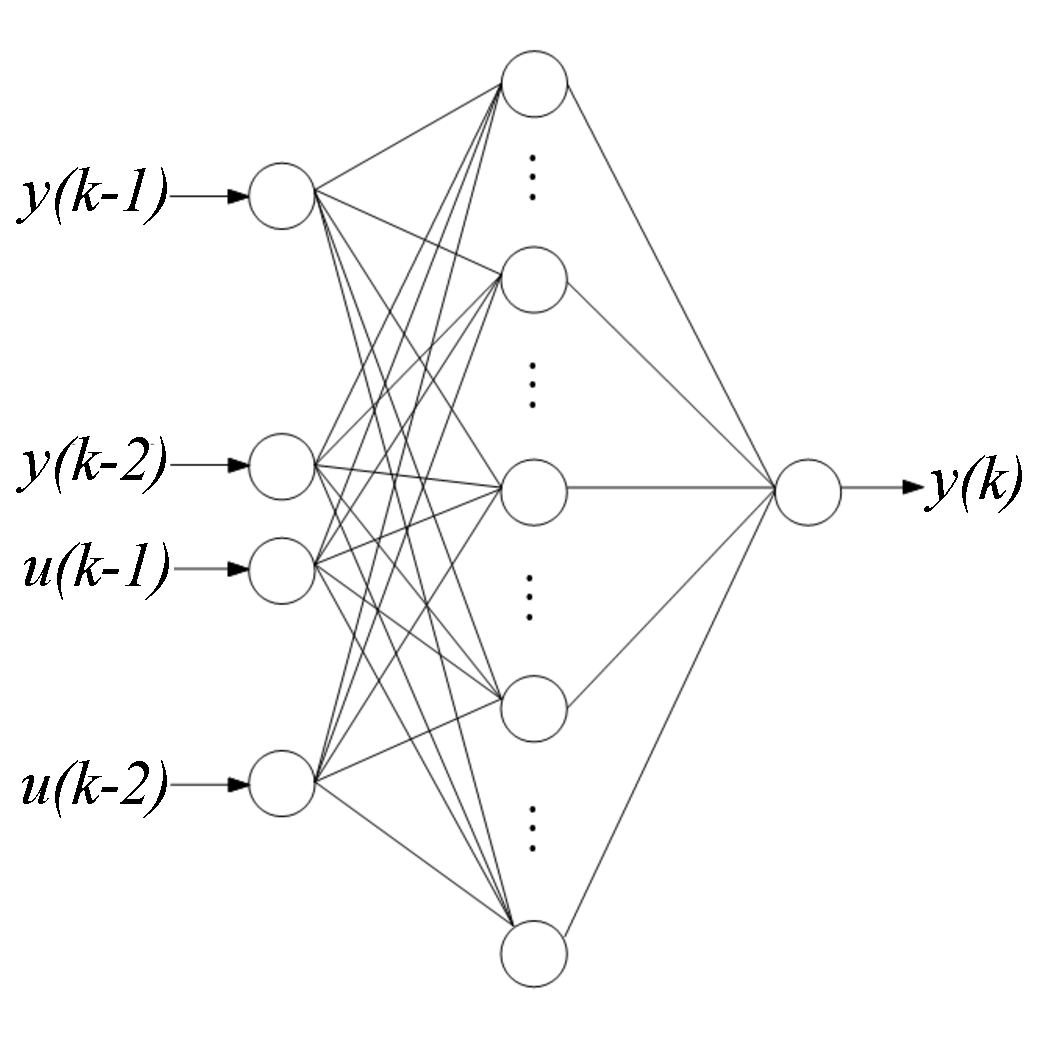
\includegraphics[width=8cm]{imag/redes/estructura.eps}
		\caption{Estructura de la red neuronal perceptrón}
		\label{estred}
	\end{figure}
	\begin{align}
	\hat{y}(k) = \sum_{i=1}^{N_h} rw_i \left( \tanh\left(\sum_{j=1}^{N_I} lw_{ji} x_j + b_i\right)\right) + c
	\label{mat_red}
	\end{align}
	
	donde, $N_h$ es el número de neuronas en la capa oculta, $N_I$ es el número de variables en la entrada, $rw_i$ es el peso que conecta la $i$-ésima neurona de la capa oculta con el nodo de salida y $lw_{ji}$ corresponde al peso que una la entrada $j$ con la $i$-ésima neurona en la capa oculta. Los sesgos de cada neuronas en la capa oculta y para el nodo de salida son $b_i$ y $c$ respectivamente.
	
	
	\item \textbf{Selección de entradas relevantes:} De los 4 regresores presente en el sistema se debe analizar cuál tiene mayor peso en el modelo. Un método para encontrar dichos regresores es mediante un análisis de sensibilidad evaluando la derivada de la salida de la red por cada premisa de nuestros datos, es decir,
	
	\begin{align}
	\xi_j = \frac{\partial \hat{y}(k)}{\partial x_j}		
	\end{align}
	Como la funcion de activacion es $tanh$ y en la salida es lineal, se tiene,
	\begin{align}
	\xi_j &= \frac{\partial \hat{y}(k)}{\partial x_j} \nonumber \\
	&= \sum_{i=1}^{Nh} rw_i \left(1 - \tanh\left(\sum_{k=1}^{N_I} lw_{ki} x_k + b_i\right)^2 \right) lw_{ji}		
	\end{align}
	
	Como se tendrá un valor de $\xi_j$ para cada dato vector de entrada, se genera un vector $\boldsymbol{\xi_j}$ del mismo largo que el número de datos de cada variable.
	
	Luego, se hace uso de un \textit{indicador} $I_j$ para cada entrada $j$ definido como,
	\begin{align}
	I_j = \mu^2 (\boldsymbol{\xi_j}) + \sigma^2(\boldsymbol{\xi_j})
	\end{align}
	donde $\mu$ es la media del vector de datos y $\sigma^2$ es la varianza para cada entrada $j$.
	
	\item \textbf{Optimizan paramétrica y estructural:} Para encontrar los valores óptimos de las parámetros peso y sesgo de la red neuronal se utiliza el algoritmo de Levenberg-Marquardt backpropagation \cite{matlab_train}. Por otro lado, para encontrar el óptimo de la estructura se analiza cuantas neuronas debe tener la capa oculta. Para ello se evalúa el RMSE (Raíz del error cuadrático medio) del conjunto de prueba en la salida de la red para un número de neuronas entre $[2-41]$. Los resultados de sensibilidad para cada neurona en la capa oculta se muestran en las Figura \ref{sensi_red_1} y \ref{sensi_red_2} y el RMSE evaluado en los 3 conjuntos se muestra en la Figura \ref{RMSE_full}. Se puede ver que el mínimo RMSE para el conjunto de prueba es para $8$ neuronas y que el modelo es menos sensible  a la entrada $u(k-2)$ el cual es eliminado del entrenamiento.
	
	\textbf{Nota:} El entrenamiento se configura a una velocidad inicial de aprendizaje de la red de $0.05$ y un valor de épocas de 4000 con evaluación de \textit{Overfitting} de 50 épocas de validación.
	
	\begin{figure}[h!]
		\centering
		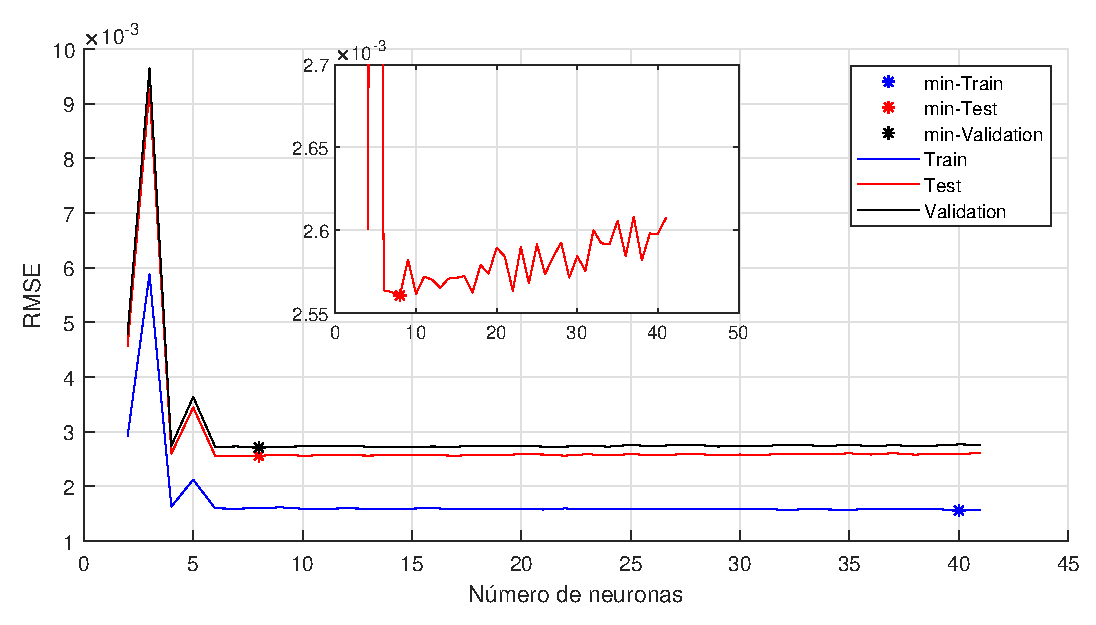
\includegraphics[width=0.8\textwidth]{imag/redes/RMSE_full.eps}
		\caption{RMSE para diferente número de neuronas.}
		\label{RMSE_full}
	\end{figure}
	\clearpage
	\begin{figure}[t!]
		\centering
		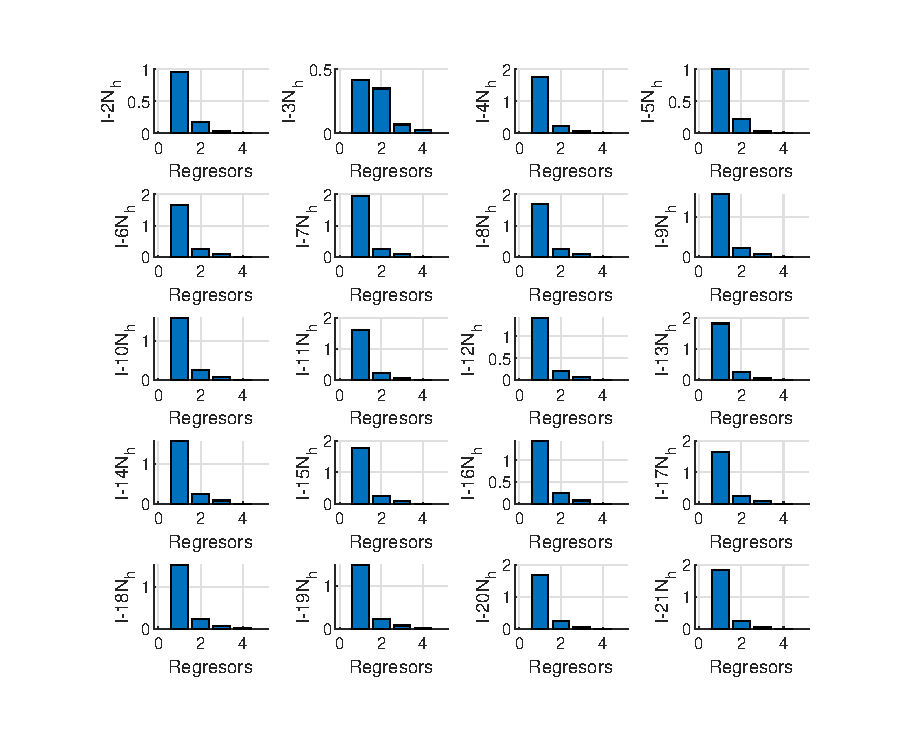
\includegraphics[width=0.8\textwidth]{imag/redes/sensibilidad_full_1.eps}
		\caption{Sensibilidad para un número de neuronas entre $[2-21]$ en la capa oculta.}
		\label{sensi_red_1}
		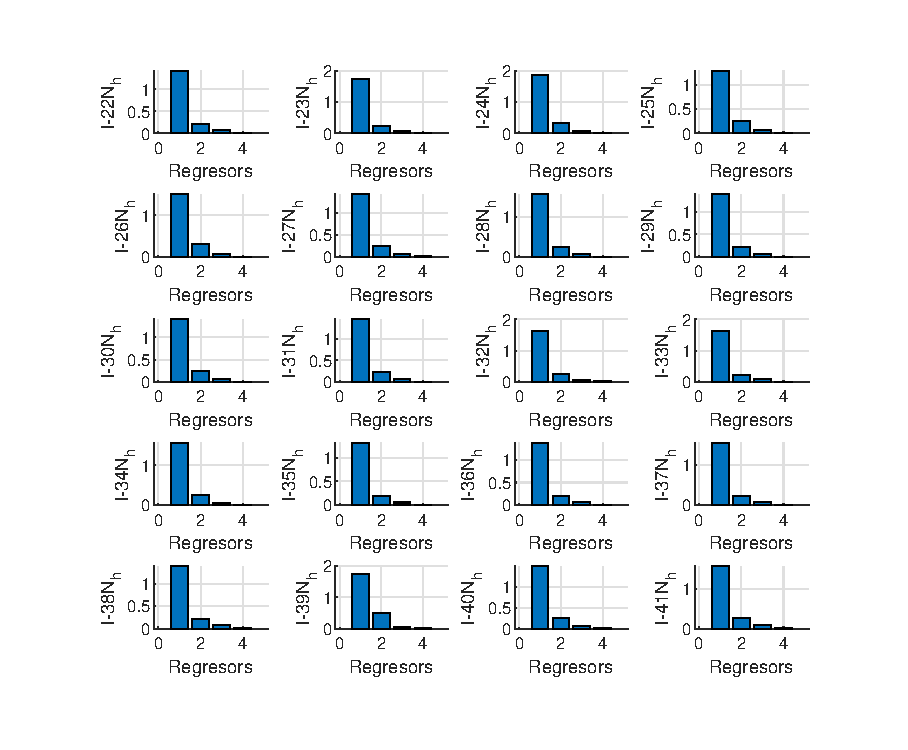
\includegraphics[width=0.8\textwidth]{imag/redes/sensibilidad_full_2.eps}
		\caption{Sensibilidad para un número de neuronas entre $[22-41]$ en la capa oculta.}
		\label{sensi_red_2}
	\end{figure}
	
	\clearpage
	
	\item \textbf{Desempeño de la red definida}: Se procede a evaluar el desempeño de la red con 8 neuronas en la capa oculta utilizando las cuatro entradas y luego solo con 3, $[y(k-1), y(k-2), u(k-1)]$, para notar las diferencias.
	Los resultados se muestran en las Figuras \ref{Ind_4} hasta la \ref{hist_4} y las datos numéricos se agrupan en la Tabla \ref{tabla_red_4_3}
	
	\begin{table}[h!]
		\centering
		\captionsetup{justification=centering}
		\caption{Valores MSE para los 3 conjuntos de datos evaluados en una red con 4 entradas y otra con 3 entradas.}
		\begin{tabular}{|l|c|c|c|}
			\hline
			Número de entradas & \multicolumn{1}{l|}{MSE - Entrenamiento} & \multicolumn{1}{l|}{MSE - Prueba} & \multicolumn{1}{l|}{MSE - Validación} \\ \hline
			4                  & 0.0084                                   & 0.0099                            & 0.0090                                \\ \hline
			3                  & 0.0149                                   & 0.0168                            & 0.0163                                \\ \hline
		\end{tabular}
	\label{tabla_red_4_3}
	\end{table}

	\begin{figure}[h!]
		\centering
		\captionsetup{justification=centering}
		\subfloat[4 Entradas]{
		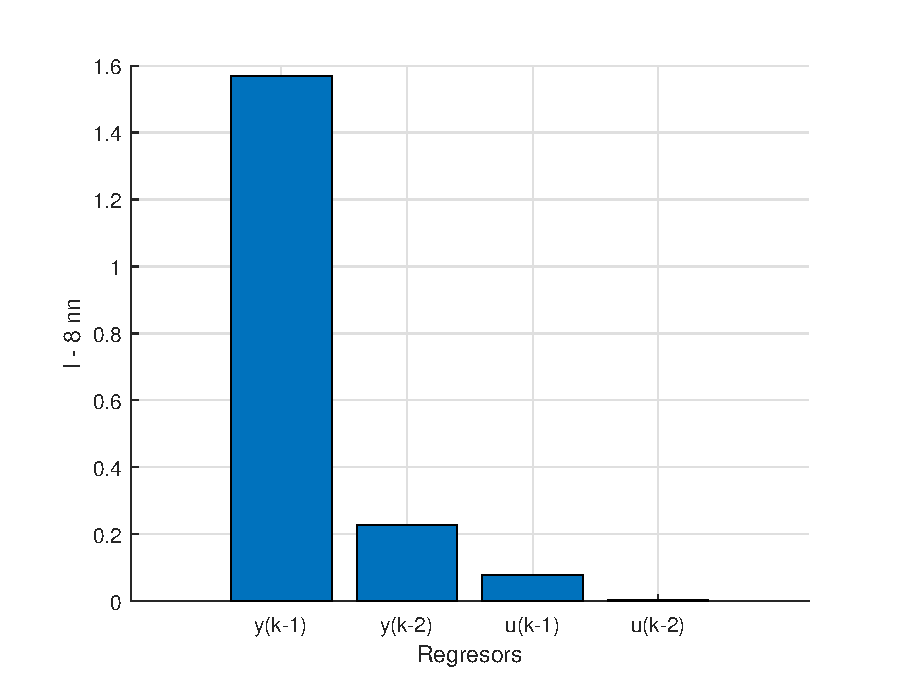
\includegraphics[width=0.5\textwidth]{imag/redes/I_4.eps}}
		\subfloat[3 Entradas]{
		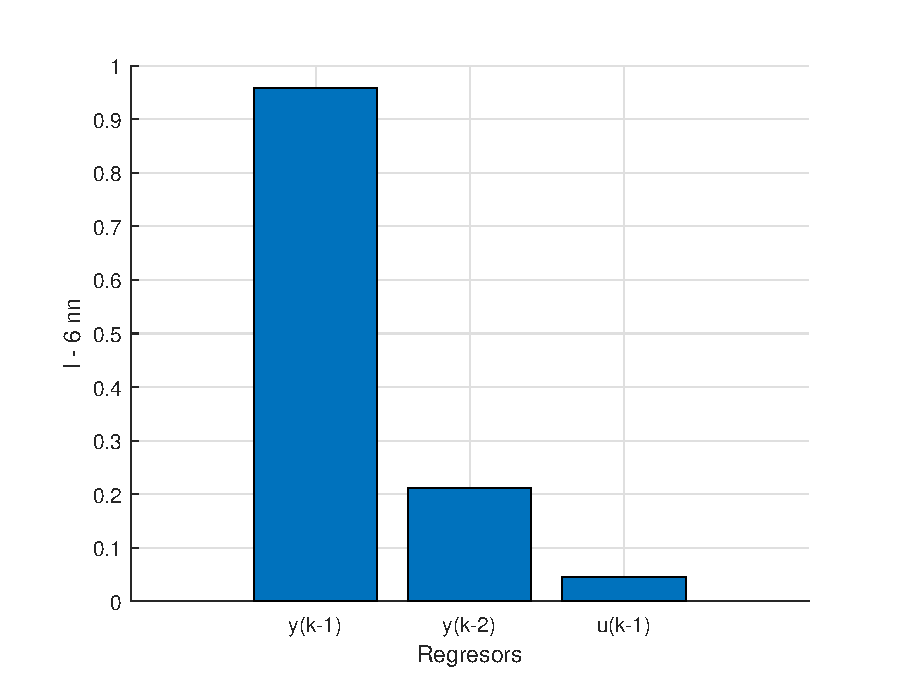
\includegraphics[width=0.5\textwidth]{imag/redes/I_3.eps}}
		\caption{Indice de sensibilidad para 4 y 3 entradas.}
		\label{Ind_4}
	\end{figure}
	Se puede notar de la Figura \ref{Ind_4} que al quitar la entrada $u(k-2)$ aumenta el indicador $I_1$ de la entrada $y(k-1)$ para compensar manteniendo casi al mismo valor las otras dos entradas. Por otro lado, no se eliminan más entradas dado que el ancho del histograma de la Figura \ref{hist_4}(b) comienza a aumentar de valor mostrando que más datos tienen errores grandes. Este error puede tener solución al utilizar un nuevo número de neuronas en la capa oculta, por lo tanto, en el siguiente ítem se procede nuevamente a encontrar el numero optimo de neuronas con 3 entradas.

	\begin{figure}
		\centering
		\captionsetup{justification=centering}
		\subfloat[4 Entradas]{
		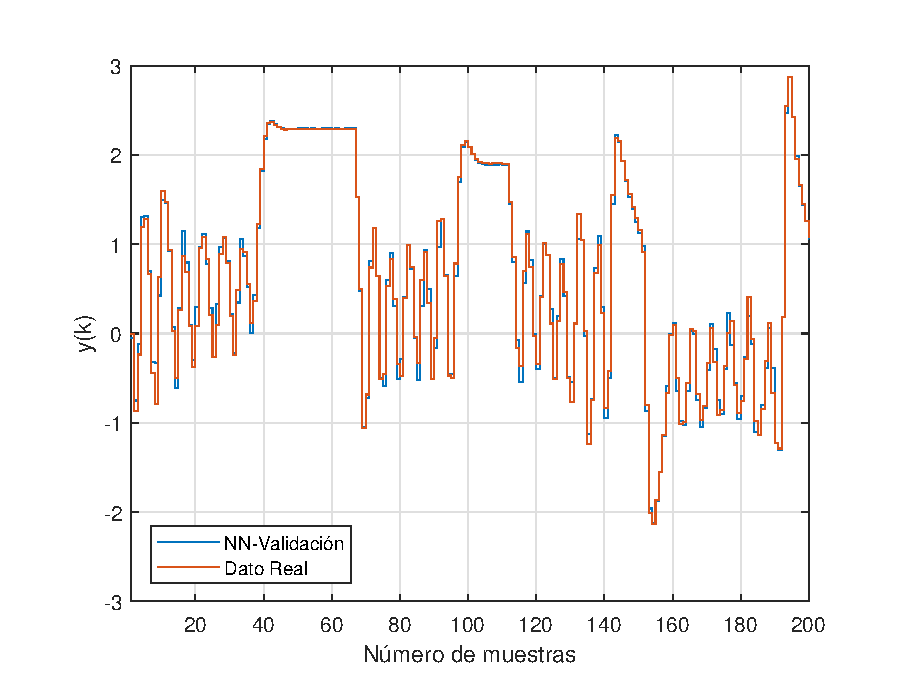
\includegraphics[width=0.5\textwidth]{imag/redes/y_red_4.eps}}
		\subfloat[3 Entradas]{
		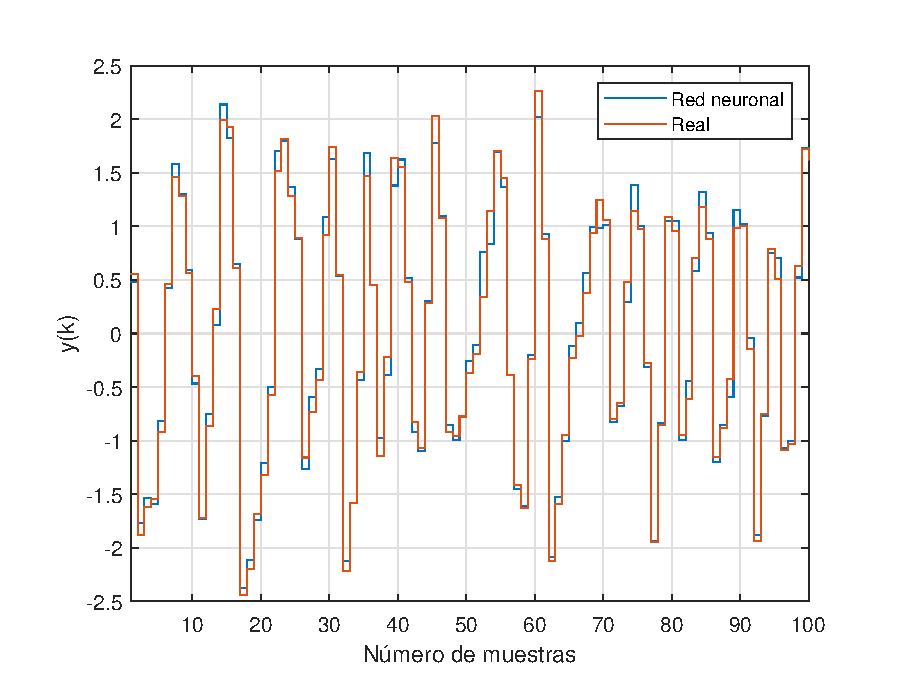
\includegraphics[width=0.5\textwidth]{imag/redes/y_red_3.eps}}
		\caption{Comparación entre la salida de la red neuronal y el valor real del conjunto de validación.}
	\end{figure}
	\begin{figure}
		\centering
		\captionsetup{justification=centering}
		\subfloat[4 Entradas]{
		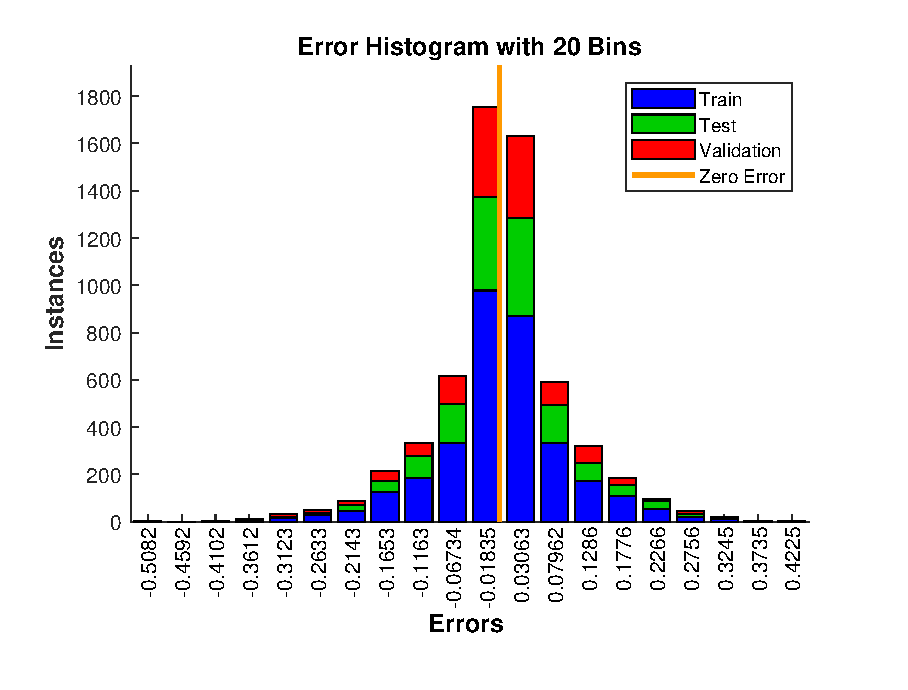
\includegraphics[width=0.5\textwidth]{imag/redes/error_4.eps}}
		\subfloat[3 Entradas]{
		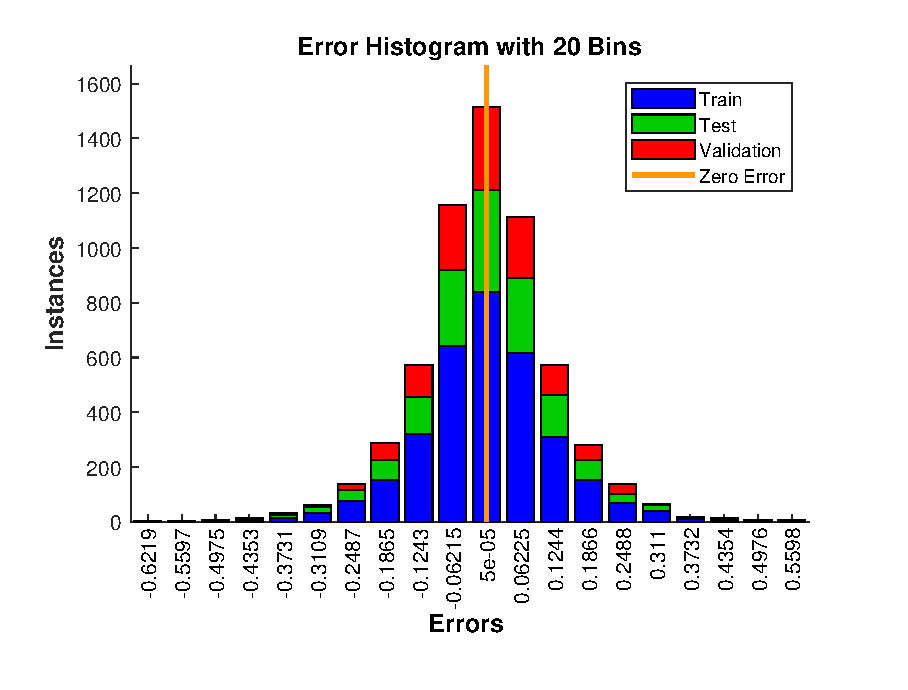
\includegraphics[width=0.5\textwidth]{imag/redes/error_3.eps}}
		\caption{Histograma del error de cada conjunto de datos.}
		\label{hist_4}
	\end{figure}

	\newpage
	\item \textbf{Optimizan estructural 2:} Se busca el número de neuronas óptimo en un rango de $[2-41]$. El resultado de la curva RMSE se muestra en la Figura \ref{rmse_3} y el análisis de sensibilidad para cada neurona en las Figuras \ref{sensi_red_1_3} y \ref{sensi_red_2_3}.

	\begin{figure}[h!]
		\centering
		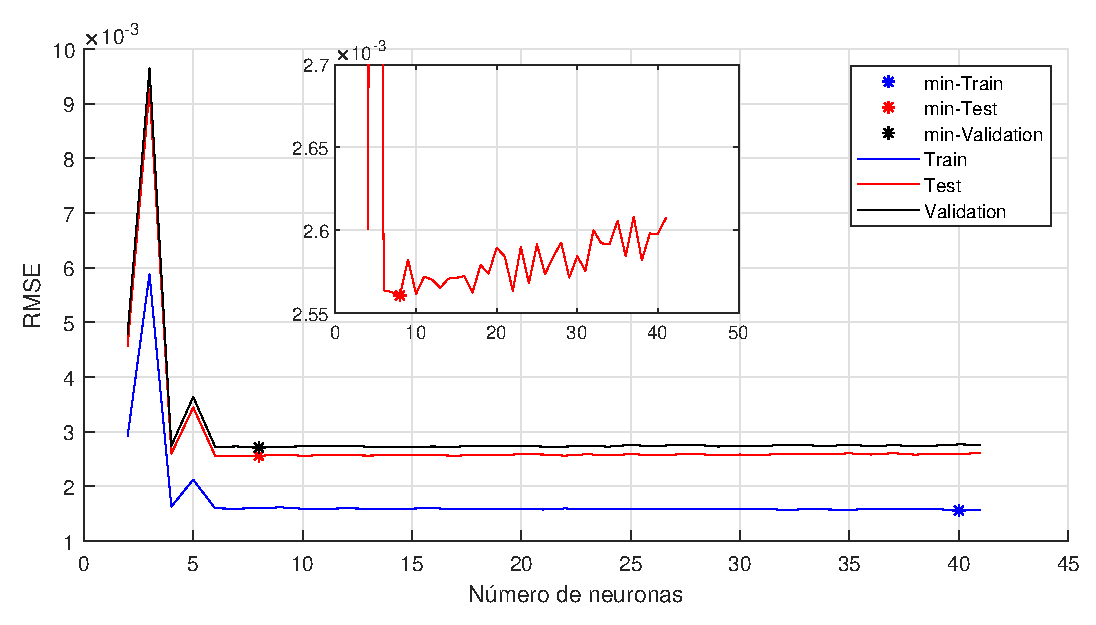
\includegraphics[width=0.8\textwidth]{imag/redes/RMSE_full.eps}
		\caption{RMSE para diferente número de neuronas.}
		\label{rmse_3}
	\end{figure}
	\newpage
	\clearpage
	\begin{figure}[t!]
		\centering
		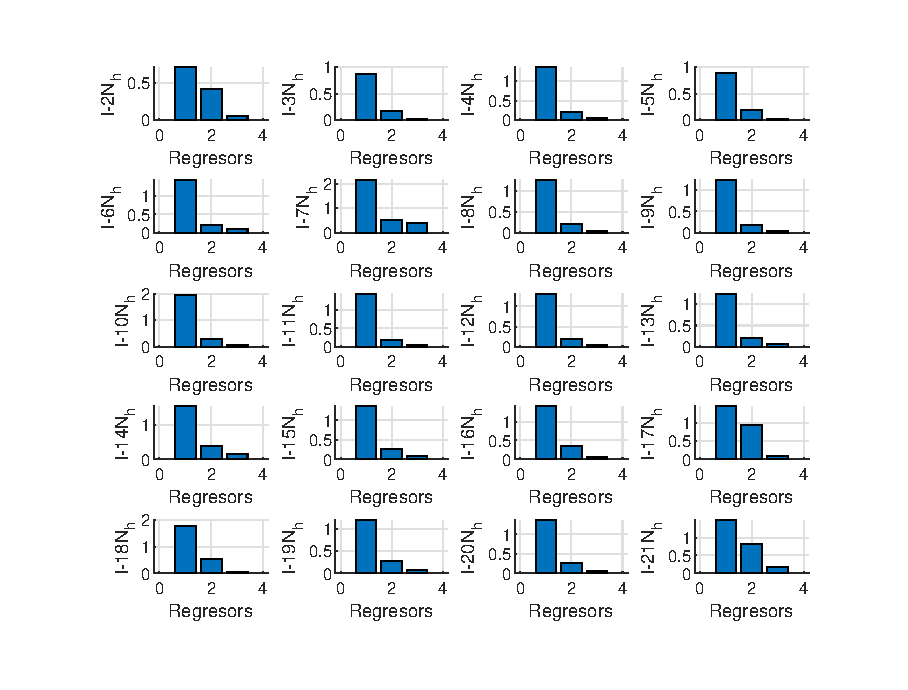
\includegraphics[width=0.8\textwidth]{imag/redes/sensibilidad_full_1_3.eps}
		\caption{Sensibilidad para un número de neuronas entre $[2-21]$ en la capa oculta.}
		\label{sensi_red_1_3}
		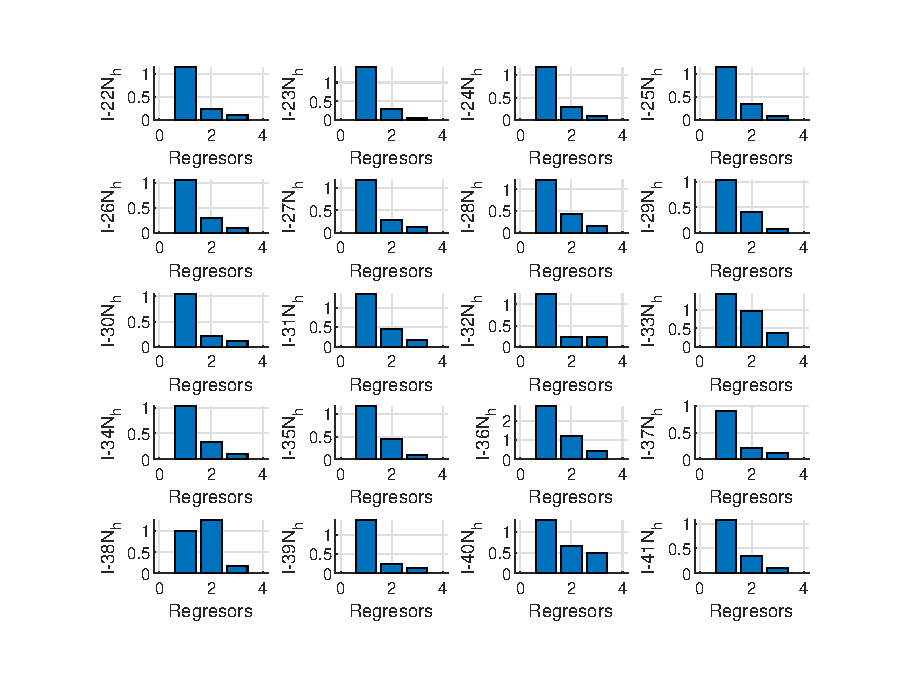
\includegraphics[width=0.8\textwidth]{imag/redes/sensibilidad_full_2_3.eps}
		\caption{Sensibilidad para un número de neuronas entre $[22-41]$ en la capa oculta.}
		\label{sensi_red_2_3}
	\end{figure}
\end{itemize}



%\section{Problema 2}
%Para la operación óptima de las micro-redes es importante contar con modelos de predicción confiables de variables tales como: potencia solar, potencia eólica, consumo, estado de carga de las baterías, entre otras variables. Los modelos e intervalos de predicción son importantes debido a la incertidumbre asociada a la generación con energía renovable y la variabilidad del consumo local.
%
%Por tal razón, se le ha confiado a usted el proyecto de determinar modelos de predicción para la generación de energía en un sistema fotovoltaico instalado en una cierta comunidad del norte del país. La finalidad de este proyecto es la de disponer de información futura de generación fotovoltaica, para así poder gestionar el funcionamiento del resto de los elementos que componen a la micro-red.
%
%Para esto se le entregarán datos históricos de generación fotovoltaica (expresada en KW) medida en la comunidad durante el periodo septiembre-diciembre de los años 2015 y 2017. Estos datos tienen un tiempo de muestreo de 1 hora (considerar porcentajes adecuados de los datos en las fases de training, test y validación).
%
%Como usted sabe, son varias las formas que se pueden emplear para la modelación a partir de estos datos, por lo que debe seleccionar el tipo de modelo más adecuado para dicha aplicación.
%
%Se sugiere considerar los datos del año 2015 como base de entrenamiento y las mediciones del año 2017 como base de prueba y validación. Para este trabajo se le pide detallar la metodología utilizada para:
%
%\begin{enumerate}[a)]
%  \item Obtener dos modelos de predicción (a elección entre los vistos en este curso) y evaluar las predicciones a 1, 6 y 12 pasos. Comparar el desempeño de todos los modelos a partir de las métricas más apropiadas tales como RMSE, MAPE, MAE, entre otras.
%  \item Construir un intervalo de predicción para los modelos obtenidos en a), utilizando método que ud. seleccione.
%\end{enumerate}
%
%\subsection{Selección de Datos}
%Se cuenta con los datos históricos de generación fotovoltaica (expresada en KW) medida en la comunidad durante el periodo septiembre-diciembre de los años 2015 y 2017. Para la selección de los conjuntos de entrenamiento, prueba y validación se utiliza una división $[60\%,20\%,20\%]$, tomándose en este caso 2160 muestars del año 2015 para entrenamiento, que corresponde a 90 días de simulaciones, y para prueba y validación 720 muestras del año 2017, el equivalente a 30 días.


\newpage
\clearpage
\section{Resultados}


\newpage
\section{Conclusión}


\newpage
\bibliographystyle{IEEEtran}
\bibliography{biblio}
\end{document} 